\documentclass[12pt,a4paper]{article}
\usepackage[margin=2.5cm]{geometry}
\usepackage{setspace}
\usepackage{titlesec}
\usepackage{braket}   % For \ket, \bra, \braket commands
\usepackage{amsmath}
\usepackage{tikz}
\usepackage{enumitem}
\usetikzlibrary{positioning, shapes.geometric, arrows.meta} % Fixed libraries

% Load hyperref only once, with all desired options
\usepackage[colorlinks=true, linkcolor=blue, urlcolor=blue, citecolor=blue, bookmarks=true]{hyperref}

% TikZ styles
\tikzset{
    startstop/.style={rectangle, rounded corners, minimum width=3cm, minimum height=1cm,
                      text centered, draw=black, fill=gray!20, align=center},
    process/.style={rectangle, minimum width=3cm, minimum height=1cm,
                    text centered, draw=black, fill=blue!20, align=center},
    arrow/.style={thick,->,>=Stealth} % Fixed arrow tip
}

% Title spacing
\titlespacing*{\section}{0pt}{2ex plus 1ex minus .2ex}{1ex plus .2ex}

\begin{document}

% ---------------- Title Page ----------------
\begin{titlepage}
    \centering
    \vspace*{2cm}

    {\LARGE \textbf{Internship Report:}}\\[1.5cm]

    {\Huge \textbf{Quantum protocol for arbitrary phase transformation}}\\[2cm]

    {\Large Ashish Nandan}\\[0.5cm]
    {\large Institute of Applied Physics, Friedrich Schiller University Jena, 07745 Jena, Germany}\\
    
    {\large date}\\[2cm]

    \textbf{Supervisors:}\\[0.5cm]
    Siavash Davani\\
    Institute of Applied Physics, Friedrich Schiller University Jena, 07745 Jena, Germany\\
    Max Planck School of Photonics, 07745 Jena, Germany\\[0.5cm]
    
    Prof. Martin Garttner\\
    Abbe Center of Photonics, Friedrich Schiller University Jena, 07745 Jena, Germany\\[0.5cm]

    Dr. Falk Eilenberger\\
    Institute of Applied Physics, Friedrich Schiller University Jena, 07745 Jena, Germany\\
    Max Planck School of Photonics, 07745 Jena, Germany\\
    Fraunhofer Institute for Applied Optics and Precision Engineering IOF, 07745 Jena, Germany

    \vfill
\end{titlepage}

% ---------------- Abstract ----------------
\section*{Abstract}
In this project we implement a programmable quantum protocol and simulate the application of arbitrary phase transformations on quantum states efficiently.
We apply a phase of our choice on a statevector using an ancilla register as a controller and analyze the resulting fidelity and error.
\[
|\psi'\rangle = \psi(x) \, e^{i \alpha |\phi(x)|^2} \, |x\rangle
\]
Here $e^{i \alpha |\phi(x)|^2}$ is the phase factor that we want to apply and can be manipulated for different phases. The primary and ancilla registers are initialized using Matrix Product States (MPS), and after that we use controlled-phase operations over multiple iterations.

\newpage

% ---------------- Contents ----------------
\tableofcontents

\newpage

% ---------------- Sections ----------------
\section{Introduction}
In quantum mechanics, phase plays a crucial role in determining interference patterns and quantum state evolution.

\newpage

\section{Theory}
We will look into the theory into three simples steps as below:

\begin{center}
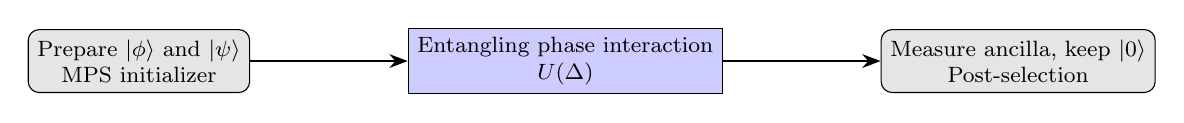
\begin{tikzpicture}[node distance=2cm, every node/.style={font=\footnotesize, align=center}]

% Nodes (smaller)
\node (prepare) [startstop, minimum width=1cm, minimum height=0.8cm] 
    {Prepare $\ket{\phi}$ and $\ket{\psi}$\\ MPS initializer};
\node (entangle) [process, right=of prepare, minimum width=1cm, minimum height=0.8cm] 
    {Entangling phase interaction \\ $U(\Delta)$};
\node (measure) [startstop, right=of entangle, minimum width=1cm, minimum height=0.8cm] 
    {Measure ancilla, keep $\ket{0}$ \\ Post-selection};

% Arrows
\draw [arrow] (prepare) -- (entangle);
\draw [arrow] (entangle) -- (measure);

\end{tikzpicture}
\end{center}
%initilization --------------
\subsection{Initialization}

Initilization is one of te major challanges in preparation of quantum circuit. A single qubit only has two amplitudes to set, but for $n$ qubits, a general state is a superposition over $2^n$ basis states, each with its own complex amplitude. To prepare a state $\ket{\psi}$ starting from $\ket{0\cdots 0}$, one would need a unitary $U$ such that
\[
U \ket{0\cdots 0} = \ket{\psi}.
\]
For highly entangled or complex states, designing such a unitary directly would require an exponentially large number of gates, which is infeasible, especially on real hardware, where noise and decoherence further complicate the process. This problem is solved by mps\_initilizer here.The MPS representation captures the essential structure of such states as a sequence of smaller matrices rather than storing all $2^n$ amplitudes explicitly. 
By using the MPS initializer, the quantum state can be constructed efficiently, piece by piece, bypassing the exponential complexity problem for states of limited entanglement.
This allows one to prepare a meaningful initial state in a circuit or simulator without having to implement a massive and impractical unitary.

In our context the ancilla register $\ket{\phi}$ is supposed to encode the phase profile $\phi(x)$. Without a proper initialization, the ancilla would remain in $\ket{0}$, carrying no information about the phase to be applied. By initializing $\ket{\phi}$ using a Matrix Product State (MPS), we efficiently encode the amplitude information of $\phi(x)$ into the ancilla register. Similarly, the primary register $\ket{\psi}$ can be initialized via MPS if it is in a nontrivial state, such as a structured wavefunction, to ensure the simulation accurately represents the starting condition.

\newpage
%Oracle----------
\subsection{Oracle $U(\Delta)$}

After initialization, comes the heart of the whole protocal, $U(\Delta)$ i.e oracle. The oracle is designed in such a way that is applies phase on the primary register $\ket{\psi}$ based on the ancilla register $\ket{\phi}$ which acts as a controller. We can contral the applied phase because the phase applied depends upon the sttae of $\ket{\phi}$. As changing the state of $\ket{\phi}$ can change $e^{i\alpha \lvert \phi(x)\rvert^2}$ which changes the output.
\setlength{\parskip}{1em}
Mathematically oracle can be defned as 
\[
U(\Delta) \;=\; I \otimes I \;+\; (e^{i\Delta} - 1) \sum_x P_x \otimes P_x ,
\]
where 
\[
P_x = \ket{x}\bra{x}, 
\qquad 
e^{i\Delta} - 1 = 2 i e^{i\Delta/2} \sin\!\left(\tfrac{\Delta}{2}\right).
\]
So the operator appears as the identity plus a projector onto the diagonal subspace 
$\sum_x P_x \otimes P_x$ weighted by that phase factor. We can see that for samll $\Delta$ we can expand
\[
U(\Delta) = I \otimes I + i \Delta \sum_x P_x \otimes P_x + \mathcal{O}(\Delta^2).
\]
This shows that $U(\Delta)$ is a weak, conditional phase kick on the subspace and only applicable when the two 
registers hold the same index.

\setlength{\parskip}{1em}
In my implementation, I follow the scalable construction described in the paper: for each bit position $j = 0, \dots, n-1$, I compare the corresponding qubits of the two registers and store an ``equal/not-equal'' flag in ancilla qubits (or compute the flags in another equivalent way). Once these flags are in place, I apply a single multi-controlled phase gate that triggers only when all flags indicate equality, and then I uncompute the flags to reset the ancillas.  

Concretely, I first compute per-qubit flags that tell me whether each bit-pair matches. The appendix of the paper gives one method using CNOT-like gates and their variants; depending on the comparator I use, the flags can indicate equality or inequality. Next, I apply an $n$-controlled phase gate $P(\Delta)$, which applies the global phase $e^{i\Delta}$ only when the entire string matches. Finally, I uncompute the flags so that the ancillas return to their clean state.  

Because the multi-controlled phase can be decomposed into $\mathcal{O}(n)$ elementary gates, and the flag computation/uncomputation uses $2n$ CNOT-style operations, the total gate count for $U(\Delta)$ scales as $\mathcal{O}(n)$. This makes $U(\Delta)$ efficient to implement as an oracle in terms of both gate depth and register size.

\newpage
\subsection{Measurement and Post-selection}

The third and most crucial part is measurement and readout part.When we prepare the ancilla register in initial step, we used mps\_initializer to entangle the ancilla register internally. We did it by applying by initializing in a rotated basis state 
$\ket{\phi_0} = U_\phi \ket{0}$. After the oracle acts, we will have the outcome the involves the superposition of both primary and ancila register. But we do not need ancilla in our measurnment, so we apply post selection measurnment and trace out ancilla register.
However, the measurement must be done in the computational basis $\{\ket{\mu}\}$, not in the rotated basis $\{\ket{\phi_\mu}\}$.

To overcome this, one applies the adjoint rotation $U_\phi^\dagger$ before measurement. The key observation is that 
\[
U_\phi^\dagger \ket{\phi_\mu} = U_\phi^\dagger \big( U_\phi \ket{\mu} \big) = \ket{\mu}.
\]

Thus, by applying $U_\phi^\dagger$ followed by a standard measurement in the computational basis, the outcome 
$\ket{\mu}$ is effectively equivalent to having projected onto $\ket{\phi_\mu}$ in the rotated basis.
The post-selection step involves keeping only the measurement outcome $\mu=0$, which corresponds to the ancilla being projected back onto its initial state $\ket{\phi_0}$. This ensures that the desired phase transformation is applied to the primary register $\ket{\psi}$, while all other outcomes (which would lead to incorrect transformations) are discarded. The probability of successfully obtaining the $\mu=0$ outcome can be made high by choosing a small enough $\Delta$ and repeating the process multiple times if necessary.

After post-selection, the state of the primary register takes the form
\begin{equation}
\psi'_0(x) \propto \psi(x) \left( 1 + 2 i \, e^{i \Delta / 2} \sin \frac{\Delta}{2} \, |\phi(x)|^2 \right).
\end{equation}

For the successful outcome $\mu = 0$, the ancilla is projected onto its prepared state
\begin{equation}
|\phi_0\rangle = |\phi\rangle.
\end{equation}
In this case, the data amplitudes evolve as
\begin{equation}
\psi'_0(x) \propto \psi(x) \left( 1 + 2 i \, e^{i \Delta / 2} \sin \frac{\Delta}{2} \, |\phi(x)|^2 \right).
\end{equation}

Using the small-$\Delta$ expansion
\begin{equation}
2 i \, e^{i \Delta / 2} \sin \frac{\Delta}{2} = i \Delta + \mathcal{O}(\Delta^2),
\end{equation}
we obtain
\begin{equation}
\psi'_0(x) \propto \psi(x) \left( 1 + i \Delta |\phi(x)|^2 + \mathcal{O}(\Delta^2) \right).
\end{equation}

The probability of this successful outcome is
\begin{equation}
P(0) = \sum_x |\psi(x)|^2 \left( 1 - 4 \sin^2 \frac{\Delta}{2} |\phi(x)|^2 \big[1 - |\phi(x)|^2 \big] \right) \ge 1 - \sin^2 \frac{\Delta}{2}.
\end{equation}

For all other outcomes $\mu \neq 0$, the post-measurement state of the primary register is
\begin{equation}
\psi'_{\mu \neq 0}(x) \propto \psi(x) \, \phi_\mu^*(x) \, \phi(x),
\end{equation}
which occurs with small probability and is discarded in the post-selection step.

Thus, by retaining only the cases with $\mu = 0$, we ensure that the protocol succeeds and that the ancilla has returned to its original rotated state.

\subsection{Iterations}
After a single cycle, the primary register state transforms as 
\begin{equation}
\psi(x) \mapsto \psi(x) \, e^{i \Delta |\phi(x)|^2} + O(\Delta^2),
\end{equation}
so one cycle imprints only a small phase proportional to $\Delta$. To apply the full target phase 
\begin{equation}
\psi(x) \mapsto \psi(x) \, e^{i \alpha |\phi(x)|^2},
\end{equation}
we can repeat the cycle $m$ times. Each successful cycle contributes another factor of $e^{i \Delta |\phi(x)|^2}$, so after $m$ cycles, the accumulated transformation is
\begin{equation}
\psi(x) \mapsto \psi(x) \left(e^{i \Delta |\phi(x)|^2}\right)^m = \psi(x) \, e^{i m \Delta |\phi(x)|^2}.
\end{equation}
To match the target phase, we choose $\Delta$ and $m$ such that
\begin{equation}
m \Delta = \alpha, \quad \text{or equivalently,} \quad \Delta = \frac{\alpha}{m}.
\end{equation}

Keeping $\Delta$ small is important because the success probability of one cycle is
\begin{equation}
P(0) \ge 1 - O(\Delta^2),
\end{equation}
which approaches 1 for small $\Delta$. If $\Delta$ is too large, the ancilla may collapse into $\mu \neq 0$ and corrupt the data, which is why the algorithm uses many small steps rather than one large step.  

The overall success probability after $m$ cycles is approximately
\begin{equation}
P_{\text{success}} \approx (1 - O(\Delta^2))^m \approx \exp(-O(m \Delta^2)).
\end{equation}
Substituting $m = \alpha / \Delta$ gives
\begin{equation}
P_{\text{success}} \approx \exp(-O(\alpha \Delta)).
\end{equation}
Therefore, if we desire an overall failure probability $\epsilon$, we should choose
\begin{equation}
\Delta = O\left(\frac{\epsilon}{\alpha}\right),
\end{equation}
which implies the number of iterations required is
\begin{equation}
m = \frac{\alpha}{\Delta} = O\left(\frac{\alpha^2}{\epsilon}\right).
\end{equation}

\clearpage
%Implementations and results-------------------------------------------------------


\newpage
\section{Implementation}
\subsection{Registers}

\subsubsection{Primary and Ancillary Registers}

The protocol makes use of two $n$-qubit registers: the primary (data) register and the ancillary (software) register. The primary register encodes the state of interest,
\begin{equation}
|\psi\rangle = \sum_{x=0}^{2^n-1} \psi(x)\,|x\rangle ,
\end{equation}
where $|x\rangle$ denotes computational basis states and $\psi(x)$ are the corresponding amplitudes. This register is the target of the programmable phase transformation.

The ancillary register plays the role of a quantum program. It is prepared in the state
\begin{equation}
|\varphi\rangle = \sum_{x=0}^{2^n-1} \varphi(x)\,|x\rangle ,
\end{equation}
with amplitudes $\varphi(x)$ chosen such that the squared modulus $|\varphi(x)|^2$ determines the phase factor applied to the data register. After applying the oracle $U(\Delta)$ and performing post-selection, the data amplitudes transform approximately as
\begin{equation}
\psi(x) \;\mapsto\; \psi(x)\, e^{i\alpha|\varphi(x)|^2}.
\end{equation}
Thus, the ancillary register acts as a programmable resource: its amplitude distribution encodes the phase profile that will be imprinted on the data state. Here the number of qubits $n$ in each register sets the size of these functions: an $n$-qubit ancilla can represent $2^n$ sampled values of $|\varphi(x)|^2$.

\subsubsection{Different Choices of the Ancilla State}

The form of the ancillary state $|\varphi\rangle$ determines the type of transformation realized on the data register. A few choices of ancilla shown here are : 
\begin{enumerate}[label=\alph*)]
    \item If $|\varphi(x)|^2$ is uniform, the same phase is applied to all basis states, producing only a global phase factor.
    \item If we take linearly increasing distribution of $|\varphi(x)|^2$, it generates a linear phase ramp, equivalent to a momentum shift in Fourier space.
    \item A Gaussian-like distribution (potential well) concentrates weight around certain indices $x$, leading to phases resembling a potential well.
    \item Exponential profiles of ancilla induce exponentially increasing or decreasing phases
    \item A periodic choices such as $|\varphi(x)|^2 \propto \sin^2(kx)$ produce periodic modulation.
    \item Randomly chosen amplitudes give rise to random phase factors, allowing simulation of disordered quantum systems.
 \end{enumerate}
 
\subsection{Protocol}

After preparing the primary register $\ket{\psi}$ and the ancillary register $\ket{\phi}$ using MPS initialization circuits, the programmable phase transformation is carried out iteratively. Each iteration consists of four experimental steps. 
\begin{enumerate}[label=\roman*)]
    \item Qubits of the two registers are compared with CNOT gates so that matching basis states can be flagged. 
    \item A small multi-controlled phase rotation $R_{z}(\Delta)$ is applied conditioned on all flags, thereby introducing a programmable phase kick. 
    \item The flags are uncomputed to restore the registers to their original basis. 
    \item The ancillary register is disentangled using $U_{\phi}^{\dagger}$, measured in the computational basis, and reset to $\ket{0}$. Only the measurement outcome corresponding to $\mu = 0$ is kept, ensuring that the ancilla returns to its original form and the protocol has succeeded.
\end{enumerate}

Repetition of this cycle $m$ times shows that the effective operation applied to the data register is a phase transformation of the form
\[
\psi(x) \;\mapsto\; \psi(x) \, e^{i m \Delta \, |\phi(x)|^{2}}.
\]


The process begins with the first loop, where controlled-NOT gates are applied with the $\phi$ register as the control and the $\psi$ register as the target. Unlike the usual CNOT, these gates are controlled on $\phi$ being $\ket{0}$ instead of $\ket{1}$. This effectively flips bits in $\psi$ in a way that encodes the comparison between $\psi$ and $\phi$. After this alignment, the multi-controlled phase gate is applied. This gate uses all but the last qubit of $\psi$ as controls and applies a small phase rotation on the final qubit if they are all in the $\ket{1}$ state. Because of the prior bit matching with $\phi$, this condition corresponds to $\psi$ and $\phi$ being in the same basis state, so the phase is applied selectively based on their match.

Once the phase is applied, the second loop undoes the bit-matching process by repeating the same CNOTs in reverse. This step disentangles $\psi$ and $\phi$, restoring them to their original form so that the $\phi$ register can later be uncomputed and measured without leaving behind unwanted correlations. 

Altogether, this sequence is a reversible \emph{compute–apply–uncompute} routine. It temporarily correlates $\psi$ and $\phi$, uses that correlation to control the application of the phase, and then removes the correlation to keep the registers clean.


\clearpage
\section{Results}




\clearpage
\appendix
\section*{Appendix: Derivation of Eqs.}
\addcontentsline{toc}{section}{Appendix: Derivation of Eqs.}

By definition, the oracle acts as
\begin{equation}
U(\Delta)\,|x\rangle|y\rangle =
\begin{cases}
e^{i\Delta}|x\rangle|y\rangle & x=y, \\[6pt]
|x\rangle|y\rangle & x\neq y .
\end{cases}
\end{equation}

This can be written compactly as
\begin{equation}
U(\Delta)\,|x\rangle|y\rangle =
\Big[1+(e^{i\Delta}-1)\delta_{x,y}\Big]\;|x\rangle|y\rangle .
\end{equation}

Promoting $\delta_{x,y}$ to operator form gives
\begin{equation}
\delta_{x,y} = \sum_{z} 
\langle x|z\rangle\langle y|z\rangle 
= \sum_{z} \langle x|\otimes \langle y| \;
\big(|z\rangle\otimes|z\rangle\big),
\end{equation}
so the operator is
\begin{equation}
U(\Delta) = I\otimes I \;+\; (e^{i\Delta}-1)\sum_{z} |z\rangle\langle z|\otimes|z\rangle\langle z| .
\end{equation}
\setlength{\parskip}{1em}


We begin with the oracle definition:
\begin{equation}
U(\Delta) \;=\; I \otimes I \;+\; (e^{i\Delta}-1)\sum_{x} \;|x\rangle\langle x|\;\otimes\;|x\rangle\langle x| .
\end{equation}
\begin{itemize}
    \item The first $\ket{x}\bra{x}$ acts on the data register (basis index $x$).
    \item The second $\ket{x}\bra{x}$ acts on the software register (basis index $y$).
\end{itemize}

\setlength{\parskip}{1em}

The input state of data ($\ket{\psi}$ register) and software ($\ket{\phi}$ register) is
\begin{equation}
|\Psi_{\text{in}}\rangle = \sum_{x} \psi(x)\,|x\rangle \otimes |\varphi_0\rangle .
\end{equation}

Now consider the action of $U(\Delta)$ on a fixed data component $|x\rangle$:
\begin{align}
U(\Delta)\,\big(|x\rangle \otimes |\varphi_0\rangle\big)
&= \Big(I \otimes I + (e^{i\Delta}-1)\sum_{x'} |x'\rangle\langle x'|\otimes |x'\rangle\langle x'|\Big)\,
\big(|x\rangle \otimes |\varphi_0\rangle\big) \\[6pt]
&= |x\rangle \otimes |\varphi_0\rangle \;+\;
(e^{i\Delta}-1)\,|x\rangle \otimes \big(|x\rangle\langle x|\,|\varphi_0\rangle\big) .
\end{align}

We can now factor out $|x\rangle$:
\begin{equation}
= |x\rangle \otimes \Big( \big[I + (e^{i\Delta}-1)\,|x\rangle\langle x|\big]\,|\varphi_0\rangle \Big).
\end{equation}

Thus, defining
\begin{equation}
U_x \;=\; I + (e^{i\Delta}-1)P_x, 
\qquad P_x = |x\rangle\langle x| ,
\end{equation}
we obtain
\begin{equation}
U(\Delta)\,\big(|x\rangle \otimes |\varphi_0\rangle\big)
= |x\rangle \otimes \big(U_x|\varphi_0\rangle\big).
\end{equation}

Finally, by expanding the full input state we find
\begin{equation}
|\Psi_{\text{out}}\rangle = \sum_{x} \psi(x)\,|x\rangle \otimes \big(U_x|\varphi_0\rangle\big).
\end{equation}
\clearpage


\newpage
\section*{Appendix: b}

Let \(U_\varphi\) be an ancilla initializer such that \(U_\varphi|\mu\rangle=|\varphi_\mu\rangle\); in particular \(|\varphi_0\rangle\equiv|\varphi\rangle\). The joint state after applying the circuit \(I\otimes U_\varphi^\dagger\; U(\Delta)\; I\otimes U_\varphi\) to \(|\psi\rangle\otimes|0\rangle\) is
\begin{align}
|\Gamma\rangle
&= \big(I\otimes U_\varphi^\dagger\big)U(\Delta)\big(I\otimes U_\varphi\big)\,|\psi\rangle|0\rangle
\nonumber\\
&= \sum_x P_x \otimes \big(U_\varphi^\dagger U_x U_\varphi\big)\;|\psi\rangle|0\rangle .
\tag{B1}
\end{align}
Measuring the ancilla in the computational basis with outcome \(\mu\) yields (unnormalized)
\[
|\psi'_\mu\rangle \propto \big(I\otimes\langle\mu|\big)|\Gamma\rangle
= \sum_x \psi(x)\,\langle\mu|U_\varphi^\dagger U_x U_\varphi|0\rangle\,|x\rangle ,
\tag{B2}
\]
where \(\psi(x)=\langle x|\psi\rangle\). Using \(|\varphi_\mu\rangle=U_\varphi|\mu\rangle\) and \(|\varphi_0\rangle=|\varphi\rangle\),
\[
\langle\mu|U_\varphi^\dagger U_x U_\varphi|0\rangle = \langle\varphi_\mu|U_x|\varphi_0\rangle.
\]
With \(U_x = I + 2i e^{i\Delta/2}\sin(\tfrac{\Delta}{2})P_x\) one obtains
\[
\langle\varphi_\mu|U_x|\varphi_0\rangle
= \langle\varphi_\mu|\varphi_0\rangle
+ 2i\,e^{i\Delta/2}\sin\!\Big(\tfrac{\Delta}{2}\Big)\langle\varphi_\mu|P_x|\varphi_0\rangle.
\tag{B3}
\]
Writing \(\varphi_\mu(x)=\langle x|\varphi_\mu\rangle\) gives \(\langle\varphi_\mu|P_x|\varphi_0\rangle=\varphi_\mu^*(x)\varphi_0(x)\), so
\[
\langle\varphi_\mu|U_x|\varphi_0\rangle
= \langle\varphi_\mu|\varphi_0\rangle
+ 2i\,e^{i\Delta/2}\sin\!\Big(\tfrac{\Delta}{2}\Big)\varphi_\mu^*(x)\varphi_0(x).
\]
For the ``good'' measurement outcome \(\mu=0\) (so \(|\varphi_0\rangle=|\varphi\rangle\)), \(\langle\varphi_0|\varphi_0\rangle=1\) and
\[
\psi'_0(x)\propto \psi(x)\Big[1+2i\,e^{i\Delta/2}\sin\!\Big(\tfrac{\Delta}{2}\Big)\,|\varphi(x)|^2\Big].
\tag{B4}
\]
The probability of obtaining \(\mu=0\) is
\[
P(0)=\sum_x |\psi(x)|^2\Big|1+2i\,e^{i\Delta/2}\sin\!\Big(\tfrac{\Delta}{2}\Big)\,|\varphi(x)|^2\Big|^2,
\]
which simplifies to
\begin{equation}
P(0)=\sum_x |\psi(x)|^2\Big(1-4\sin^2\!\tfrac{\Delta}{2}\,|\varphi(x)|^2\big(1-|\varphi(x)|^2\big)\Big).
\tag{B5}
\end{equation}
Using \( |\varphi(x)|^2(1-|\varphi(x)|^2)\le\tfrac14\) we obtain the lower bound
\[
\boxed{ \; P(0)\ge 1-\sin^2\!\Big(\tfrac{\Delta}{2}\Big) \; } \tag{B6}
\]
so for small \(\Delta\) the success probability is close to unity.

\bigskip
\textbf{Remarks.}
\begin{itemize}
  \item For \(\Delta\ll1\), \(2i e^{i\Delta/2}\sin(\Delta/2)\approx i\Delta\), so the per-cycle factor in (B4) approximates \(e^{i\Delta|\varphi(x)|^2}\). Repeating \(m\) cycles with \(\Delta=\alpha/m\) approximates \(e^{i\alpha|\varphi(x)|^2}\).
  \item If \(\Delta\) is not small the \(\sin(\Delta/2)\) prefactor introduces nonlinear dependence on \(\Delta\) (oscillations), explaining non-monotonic fidelity vs.\ \(m\) when \(\alpha\) is fixed and \(\Delta=\alpha/m\) exits the small-\(\Delta\) regime.
  \item Measurement outcomes \(\mu\neq0\) are low-probability branches that lead to corrupted transformations proportional to \(\varphi_\mu^*(x)\varphi(x)\) (see B3); they are the origin of rare but damaging error events.
  \item In your circuit: \(U_\varphi\) is the MPS initializer on the ancilla, the controlled-phase/multi-controlled-phase implements the \(U(\Delta)\)-style coupling, then \(U_\varphi^\dagger\) and ancilla measurement implement the projection onto \(|\mu\rangle\).
\end{itemize}



\end{document}